\section{Introduction:}

Huffman codes compress data very effectively: savings of 20 $\%$ to 90 $\%$ are typical, depending on the characteristics of the data being compressed. We consider the data to be a sequence of characters. Huffman’s greedy algorithm uses a table giving how often each character occurs ( i.e., its frequency ) to build up an optimal way of representing each character as a binary string. Suppose we have a 100,000 - character data file that we wish to store compactly. We observe that the characters in the file occur with the frequencies given by Figure 1.0. That is, only 6 different characters appear, and the character {\bfseries a} occurs 45,000 times. We have many options for how to represent such a file of information. Here, we consider the problem of designing a binary character code ( or code for short ) in which each character is represented by a unique binary string, which we call a {\bfseries codeword}. If we use a {\bfseries fixed-length code}, we need 3 bits to represent 6 characters: {\itshape a = "000", b = "001" ... f = "101}. This method requires 300,000 bits to code the entire file. Can we do better?

\begin{figure}[H]
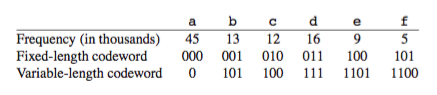
\includegraphics[height = 4cm, width = 10cm]{1.png}
\centering \linebreak \linebreak {\small Figure 1.0: A character-coding problem. A data file of 100,000 characters contains only the characters a - f, with the frequencies indicated. If we assign each character a 3 - bit codeword, we can encode the file in 300,000 bits. Using the variable-length code shown, we can encode the file in only 224,000 bits.}
\end{figure} \hfill \break

A {\bfseries variable-length code} can do considerably better than a fixed-length code, by giving frequent characters short codewords and infrequent characters long code- words. Figure 1.0 shows such a code; here the 1 - bit string 0 represents {\bfseries a}, and the 4-bit string 1100 represents {\bfseries f}. This code requires 224, 000 bits to represent the file, a savings of approximately 25$\%$. In fact, this is an optimal character code for this file, as we shall see.
\pagebreak